\documentclass{article}

\usepackage[letterpaper]{geometry}
\usepackage{graphicx}

\graphicspath{{./img/}}

\title{2411 HW 6}
\author{Duncan Wilkie}
\date{15 October 2021}

\begin{document}

\maketitle

\section*{1}
A plot of $\tan(x)-x$ on $[2,8]$ appears below.
\[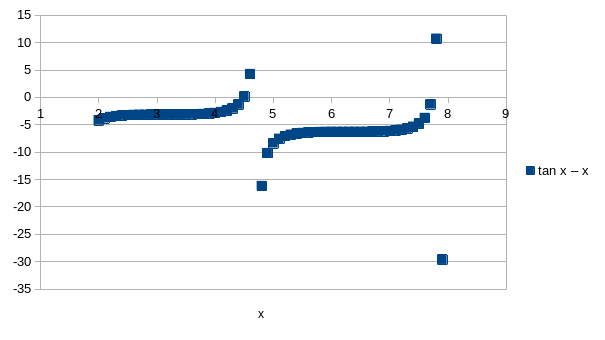
\includegraphics[scale=0.5]{plot1.png}\]
Two values of $x$ just after which the function becomes positive are $x=4.4,7.6$. These will serve as our intial guesses.
The program implementing Newton-Raphson appears in the script files section. It results in approximations for the roots of $x=4.493409458, 7.725251837$
Calculating the values $p_1, p_2$ corresponding to the $x$ found above, $p_1=\frac{x_1}{\pi}=1.4303$ and $p_2 = \frac{x_2}{\pi} = 2.45902$. These are within 5\% and 2\% of the true values of $1.5$ and $2.5$ respectively, so approximating the positions of the maxima as halfway between minima is justified.
\section*{Script Files}
\begin{verbatim}
Script started, file is dwilk14_hw6p1.txt
[dwilk14@tigers ~/HW6]$ cat dwilk14_hw6p1.cpp
#include <fstream>
#include <iostream>
#include <cmath>

using namespace std;

double f(double x) {
    return tan(x) - x;
}

double deriv(double x) {
  return pow(tan(x), 2);
}

int main() {
  ofstream outfile;
  outfile.open("output.txt");
  outfile.precision(10);
  double guess1 = 4.4,  guess2 = 7.6, fx1 = f(guess1), fx2 = f(guess2);


  outfile << "n x1 fx1" << endl;

  for (int i = 0; i < 15; i++) {
    outfile << i << " " << guess1 << " " << fx1 << endl;

    if (abs(fx1) < 1e-8) {
      break;
    }

    guess1 -= fx1 / deriv(guess1);
    fx1 = f(guess1);

  }

  outfile << "n x2 fx2" << endl;


  for (int i = 0; i < 15; i++) {
    outfile << i << " " << guess2 << " " << fx2 << endl;

    if (abs(fx2) < 1e-8) {
      break;
    }

    guess2 -= fx2 / deriv(guess2);
    fx2 = f(guess2);

  }

  return 0;

}
[dwilk14@tigers ~/HW6]$ g++ dwilk14_hw6p1.cpp -o dwilk14_hw6p1
[dwilk14@tigers ~/HW6]$ ./dwilk14_hw6p1
[dwilk14@tigers ~/HW6]$ cp dwilk14_hw6p1.txt /home3/kristina/phys2411/.
[dwilk14@tigers ~/HW6]$ exit
exit
Script done, file is dwilk14_hw6p1.txt
\end{verbatim}
\end{document}
%%% Local Variables:
%%% mode: latex
%%% TeX-master: t
%%% End:
